
\documentclass[a4paper,12pt]{article}

\usepackage[russian]{babel}
\usepackage[utf8]{inputenc}
\usepackage{cmap}
\usepackage{amsmath}
\usepackage{amssymb}
\usepackage{xspace}
\usepackage{graphicx}
\usepackage{sectsty}
\usepackage{fancyhdr}
\usepackage{longtable}
\usepackage{indentfirst}
\usepackage{url}
\usepackage{appendix}
\usepackage{enumerate}
\usepackage{totcount}
\usepackage{listings}

\newcommand{\EN}[1]{{#1}}
\newcommand{\CODE}[1]{{\ttfamily #1}}

\fancyhf{}
\fancyfoot[C]{\normalsize \thepage}
\renewcommand{\headrulewidth}{0pt}
\renewcommand{\footrulewidth}{0pt}

%%Modifying captions for figures and tables:
\makeatletter
\long\def\@makecaption#1#2{%
\vspace{\abovecaptionskip}%
\sbox{\@tempboxa}{\large #1.~#2}
\ifdim \wd\@tempboxa >\hsize
{\large #1 --- #2}\par
\else
\global\@minipagefalse
\hbox to \hsize {\hfill {\large #1 --- #2}\hfill}%
\fi
\vspace{\belowcaptionskip}}

\renewcommand{\baselinestretch}{1.2}
%%\sectionfont{\LARGE}
\sectionfont{\Large}
\subsectionfont{\Large}
\subsubsectionfont{\Large}
\setlength{\belowcaptionskip}{6pt}
\makeatletter \renewcommand{\@biblabel}[1]{#1.\hfill}

\makeatletter 
\def\redeflsection{\def\l@section{\@dottedtocline{1}{1.5em}{7.8em}}} 
\renewcommand\appendix{\par 
\setcounter{section}{0}% 
\setcounter{subsection}{0}% 
\def\@chapapp{\appendixname}% 
\addtocontents{toc}{\protect\redeflsection} 
\def\thesection{\appendixname\hspace{0.2cm}\@Asbuk\c@section}} 
\makeatother 

\textwidth = 17cm
\oddsidemargin= 0 pt
\topmargin = -1cm
\headheight = 0cm
\headsep = 0cm
\textheight = 26.5cm

\newtotcounter[auxfile=totals.aux]{figurecnt}
\def\oldfigure{} \let\oldfigure=\figure
\def\figure{\stepcounter{figurecnt}\oldfigure}
\newtotcounter[auxfile=totals.aux]{bibcnt}
\def\oldbibitem{} \let\oldbibitem=\bibitem
\def\bibitem{\stepcounter{bibcnt}\oldbibitem}
\regtotcounter[auxfile=totals.aux]{page}


\begin{document}
\def\figurename{Рисунок}
\sloppy
\lstset{language=Python} 
\normalsize
\thispagestyle{empty}
\begin{center}
МИНОБРНАУКИ РОССИИ\\
ТОМСКИЙ ГОСУДАРСТВЕННЫЙ УНИВЕРСИТЕТ\\
Факультет информатики\\
Кафедра теоретических основ информатики\\
\end{center}

\vspace{0.7cm}

УДК 681.03

\vspace{0.5cm}

\begin{flushright}
ДОПУСТИТЬ К ЗАЩИТЕ В ГАК\\
Зав.кафедрой, доцент, к.т.н.\\
\makebox[3cm]{\hrulefill}А.Л.Фукс\\
«\makebox[0.8cm]{\hrulefill}»\makebox[1.5cm]{\hrulefill}2013 г.\\
\end{flushright}



\begin{center}

\vspace{1.5cm}
{\bf БАКАЛАВРСКАЯ РАБОТА}\\
\vspace{0.5cm}
СОЗДАНИЕ инструментария ДЛЯ ТЕСТИРОВАНИЯ ЦЕЛОСТНОСТИ РЕПОЗИТОРИЯ ПАКЕТНОГО МЕНЕДЖЕРА DEEPSOLVER

\vspace{0.5cm}
по основной образовательной программе подготовки бакалавров\\
010400 --- Информационные технологии

\vspace{0.5cm}

Кирюшкина Валентина Евгеньевна


\end{center}

\vskip 0pt plus 1filll

\begin{tabbing}
\hspace{10cm}\=Руководитель ВКР, к.т.н.\\
\>\makebox[3cm]{\hrulefill}М.С.Пожидаев\\
\>«\makebox[0.8cm]{\hrulefill}»\makebox[1.5cm]{\hrulefill}2013 г.\\
\end{tabbing}

\begin{tabbing}
\hspace{10cm}\=Автор работы\\
\>студент группы №1493\\
\>\makebox[3cm]{\hrulefill}В.Е.Кирюшкина\\
\end{tabbing}

\vspace{0.8cm}

\hspace{-0.65cm}Электронная версия бакалаврской работы помещена\\
в электронную библиотеку. Файл

\vspace{1.2cm}

\begin{center}
Томск - 2013
\end{center}
\normalsize

\newpage
\begin{center}
	\textbf{Реферат}
\end{center}

Выпускная квалификационная работа \total{page}~с., \total{figurecnt}~рис., источников \total{bibcnt}.

ПАКЕТНЫЙ МЕНЕДЖЕР, ДИСТРИБУТИВ, ALTLINUX, PYTHON, SOFTWARE DEPENDENCIES.

Объект исследования --- методы разрешения зависимостей в пакетных менеджерах второго уровня.

Цель работы --- разработка утилит для проверки целостности репозитория пакетного менеджера Deepsolver.

Результаты работы --- разработаны утилиты для проверки целостности репозитория, проведен запуск
на основном репозитории Deepsolver.


\newpage
\pagestyle{fancy}
\renewcommand{\contentsname}{Оглавление}
\tableofcontents 
\newpage
\section*{Введение}
\addcontentsline{toc}{section}{\hspace{7mm}Введение}

На современные компьютеры необходимо устанавливать сотни программ в рамках
одной операционной системы. В операционной системе GNU/Linux программное 
обеспечение (ПО) распространяется в форме пакетов, тесно связанных друг с другом,
которые находятся в централизованном хранилище в сети, --- репозитории. 
Фактически, не предполагается возможности получения ПО из 
других источников, таким образом, репозиторий представляет собой хранилище 
колоссальных размеров, где пакеты тесно связаны друг с другом.

Основным свойством репозитория является целостность, что подразумевает
возможность установки пользователем любого пакета, в нем находящегося. 
Обеспечение этого свойства составляет одну из основных задач утилит для 
работы с репозиторием. 

В компании  ALT~Linux было принято решение о создании новой системы
управления пакетами  - пакетного менеджера Deepsolver, поэтому возникла 
необходимость проверки целостности репозитория данной системы, по сути, 
качества работы упомянутых утилит. 

Таким образом, целью настоящей работы является проектирование 
инструментария контроля целостности репозитория, удовлетворяющего условиям эксплуатации в~окружении ALT~Linux, 
и реализация на~базе подготовленного проекта необходимых утилит.

\newpage
\newpage
\section{Распространение ПО в ОС GNU/Linux}

В большинстве дистрибутивов \textit{GNU/Linux} программное обеспечение находится
в централизованном хранилище, чаще всего располагающемся в Интернете, 
--- \textit{репозитории}. Любой пакет в~репозитории представляет собой файл, содержащий
информацию о продукте, программные файлы и документацию, --- \textit{пакет}. 
Пакеты тесно связаны между собой: к примеру, для установки одного пакета
может потребоваться некоторое множество других, так же существуют пакеты, 
несовместимые друг с другом. 

Вспомогательная информация о пакетах, включая их связи, иначе называемые зависимостями,
хранится в репозитории и называется \textit{индексом}.
По сути, индекс представляет собой нормализованную форму для хранения информации о пакетах 
репозитория, которая становится доступна пользователю.

Если пакет предоставляет 
функциональность других пакетов, то он указывает информацию об этом в тэге \textit{provides}.
Имя \textit{provides} допускает произвольное значение, не обязательно совпадающее с
именем какого-либо реально существующего  пакета и является, скорее, соглашением, что пакет
обладает некоторой совместимостью. Для \textit{provides} допускается указание подмножества 
версии. Неявными \textit{provides} считаются имена всех файлов, хранимых в пакете.\\

Так же допустимы следующие типы отношений на множестве пакетов, информация о которых так
же содержится в индексе\cite{deepsolver_ta}:
\begin{itemize}
\item{\textit{Requires}: пакет требует обязательное наличие другого пакета, указанного
по его имени или по одному из его \textit{provides}. Допускается указание 
подмножества версии требуемого пакета. В случае указания ограничения версии
под \textit{requires} может подходить \textit{provides} только дополненный информацией
о версии.}
\item{\textit{Conflicts}: пакет запрещает наличие другого пакета, указанного по его имени
 или по одному из его \textit{provides}. Допускается указание подмножества
версии конфликтуемого пакета. В случае указания ограничения версии
под \textit{conflicts} может подходить \textit{provides} только дополненный информацией
о версии.}
\item{\textit{Obsoletes:} Пакет может указывать, что является обновлением некоторого
множества пакетов. При установке такого пакета все пакеты, обновлением
которых он является, удаляются из ОС. Попытка их установки после
установки обновляющего пакета приводит к ошибке типа ``установлена
более свежая версия''. Допускается указание подмножества версии обновляемых
пакетов. В случае указания ограничения версии под \textit{obsoletes} может
подходить \textit{provides} только дополненный информацией о версии.}
\end{itemize}

На основе анализа информации, полученной из индекса репозитория,
можно делать выводы о его состоянии. \\

Описанные выше отношения можно представить в виде математической модели,
которая будет проиллюстрирована в \ref{sn:software_dependencies_model}.

%FIXME: здесь ли моддель зависимостей?

\subsection{Пакетные менеджеры}
Так как репозиторий содержит множество пакетов, которые, помимо прочего, тесно
связаны друг с другом, существует необходимость в программном обеспечении для
корректного добавления, удаления и обновления пакетов, а так же их инсталляции.
Данные программные продукты называются пакетными менеджерами.\\

Выделяют два уровня пакетных менеджеров:
\begin{itemize}
\item{Пакетные менеджеры первого уровня предоставляют интерфейс для установки,
удаления и обновления пакетов: они позволяют проверить наличие необходимых для
работы устанавливаемой программы компонент подходящей версии непосредственно 
в момент установки, а также производят необходимые процедуры для регистрации 
программы во всех операционных средах пользователя. Например, cразу после установки 
программа может быть доступна пользователю из командной строки.}
\item{Для решения задачи инсталляции пакета, то есть осуществления поиска пакета для
установки по заданным критериям, учитывая его зависимости, применяется усовершенствованная
система управления пакетами --- пакетные менеджеры второго уровня. Менеджеры второго уровня 
являются надстройкой над менеджерами первого уровня.}
\end{itemize}

Примером пакетного менеджера первого уровня является  \textit{RPM} --- рекурсивный акроним 
\textit{RPM Package Manager}, ранее раскрывался, как \textit{Red Hat Package Manager}.
По сути, менеджером этого уровня определяется формат пакета.\\

Название rpm-пакета состоит из нескольких частей и в общем виде может быть представлено
такой строкой: \\
\textit{name-version-release.architecture.rpm}, где:
\begin{itemize}
\item{\textit{name} - имя пакета (чаще всего --- название основного приложения, содержащегося в пакете);}
\item{\textit{version} - версия}
\item{\textit{release} - релиз}
\item{\textit{architecture} - архитектура}
\end{itemize}

%FIXME:менеджеры второго уровня, раньше был apt, теперь deepsolver.рассказать про первый
Примером пакетного менеджера, работающего с rpm-пакетами, является \textit{Deepsolver}, система
управления пакетами от компании \textit{ALT Linux}.\\

\subsubsection{Пакетный менеджер Deepsolver}
Можно выделить две составные части пакетного менеджера Deepsolver:
\begin{itemize}
\item{Клиентская часть, предоставляющая интерфейс для установки, обновления
 и удаления пакетов на компьютере пользователя.}
\item{Автоматическая сборочница --- программная часть, отвечающая за сборку пакетов.
Работает она следующим образом: автор пакета присылает ссылку на \textit{git-репозиторий} с исходным кодом, %%сделать ссылку про git
после чего в строго автоматизированном порядке программа выполняет сборку пакета и кладет
его в репозиторий. Сборка может осуществляться как перед помещением пакета в репозиторий,
так и в любое другое время, если администратор решил пересобрать репозиторий.}
\end{itemize}

\paragraph{Администрирование репозитория\\} 
\textit{Deepsolver} для правильной работы требует выполнения некоторых задач 
администрирования, которые включают в себя задачи обслуживания репозиториев
пакетов и настройку \textit{Deepsolver} на рабочих местах.

Все задачи администрирования репозиториев сводятся к созданию и поддержке в
актуальном состоянии индекса репозитория, который доставляется в первую очередь на компьютеры
пользователей, от его актуальности зависит корректность обработки запросов 
на внесение изменений в состояние ОС. В простейшем варианте индекс
хранит перечисление доступных пакетов с необходимыми атрибутами, включая
полный список \textit{provides}, из-за чего размер файлов индекса становится
чрезмерно большим. Тем не менее, на практике доля \textit{provides}, действительно
задействованных в вычислении зависимостей между пакетами, невелика,
и это даёт возможность для различных оптимизаций размера хранимой информации.

Правильный подход настройки фильтрации \textit{provides} выбирается исходя
из назначения репозитория. Существуют следующие режимы:
\begin{enumerate}
\item{ Фильтрация на основе поиска соответствующих записей \textit{requires/conflicts}.\\
Если репозиторий является единственным источником пакетов для установки
на компьютеры пользователей, и нет других сторонних источников ПО, 
то эффективное сокращение количества \textit{provides} может быть
достигнуто за счёт включения режима фильтрации на основе известных
\textit{requires/conflicts}. При активации этого режима запись \textit{provides} сохраняется
в индексе только в том случае, если известна хотя бы одна запись
\textit{requires} или \textit{conflicts}, в которой имя пакета совпадает с именем пакета
в \textit{provides}. Информация о версии в этом случае не учитывается. В терминологии 
Deepsolver соответствующие записи \textit{requires/conflicts} иногда называются ``ссылками''.}
\item{ Фильтрация на основе каталогов файлов.\\
 Режим фильтрации \textit{provides} на основе информации о каталоге файла может применяться только для
тех записей \textit{provides}, которые были сгенерированы автоматически на основе
 списка файлов пакета. \textit{Deepsolver} имеет возможность указания списка
каталогов, файлы из которых всегда обрабатываются как допустимые
\textit{provides}. Эта возможность полезна для выполнения запросов на установку
 пакетов по имени файлов. Например, по имени файлов из каталога
\textit{/usr/bin}.}
\end{enumerate}
Если ни один из указанных режимов фильтрации \textit{provides} не используется,
то индекс содержит все возможные \textit{provides}. Если указаны оба из них, то
в индекс попадает \textit{provides}, если он подходит хотя бы под одно правило.

\textit{Deepsolver} предоставляет возможность внесения изменений в индекс без
полной перегенерации, что порождает ряд трудностей при использовании
фильтрации \textit{provides} на основе известных \textit{requires/conflicts}. При появлении
новых пакетов нарушается общая целостность, поскольку корректное добавление 
требует восстановления ранее исключённых \textit{provides}. Описанные ниже
утилиты позволяют правильно обновлять содержимое индекса и поддерживать
его в целостном состоянии.

\paragraph{Утилиты для работы с репозитория\\}
Для решения вышеописанных проблем используются утилиты \textit{ds-repo, ds-patch, ds-provides}\cite{deepsolver_um},
являющиееся частью упомянутой ранее программы для сборки пакетов.
В качестве одного из аргументов каждая из них требует путь к директории
 с файлами индекса.\\

\textit{ds-repo} выполняет все действия по созданию индекса для некоторой
одной компоненты репозитория. Главными параметрами для неё являются
путь к каталогу, где должен быть расположен новый индекс, и множество
путей к каталогам с пакетами, которые должны быть зарегистрированы. 
Целевой каталог создаётся автоматически. Если он уже существует, то не 
должен содержать других каталогов или файлов. 

Каталоги с пакетами могут
быть перечислены в произвольном порядке и могут содержать как бинарные
пакеты, так и пакеты с исходными текстами. Утилита \textit{ds-repo} автоматически
распознает их тип и помещает в соответствующий раздел индекса. Имена
всех описанных каталогов указываются как свободные параметры командной
строки. 

На первом месте должен быть указан целевой каталог, за которым
следует перечисление каталогов с пакетами. Пропуск целевого каталога
не допускается. Если ни один из каталогов с пакетами не указан, то 
просматривается текущий каталог, установленный на момент запуска утилиты.\\

Утилита \textit{ds-patch} производит включение и исключение файлов из построенного
индекса Deepsolver. 

Все параметры, указываемые при вызове\textit{ ds-repo},
повторно перечислять не нужно. Они сохраняются в информационном файле
индекса репозитория и загружаются автоматически при изменении его содержимого.
При запуске \textit{ds-patch} производится проверка контрольных сумм, и
если регистрируется факт обнаружения повреждённого файла, работа завершается
с ошибкой. 

После работы суммы изменённых файлов обновляются.
При использовании утилиты \textit{ds-patch} необходимо помнить, что утилита
только изменяет набор файлов, перечисленных в индексе, но не обрабатывает 
множество \textit{provides}, которое после изменения теряет целостность и
должно быть отдельно обработано утилитой \textit{ds-provides}, описанной ниже. 
Целостность списка provides нарушается не только в изменённом индексе, но и
во всех других взаимосвязанных компонентах репозитория. 

Таким образом,
для них также должна быть произведена обработка утилитой \textit{ds-provides}.
Утилита \textit{ds-patch} ожидает указания одного свободного параметра --- каталога
с индексом для изменения. Если он не указан, то используется текущий
каталог. Файлы для включения или исключения должны перечисляться после ключей
- \textit{-add} и - \textit{-del} соответственно. Файлы для включения должны быть перечислены 
с указанием абсолютного пути к файлу пакета, в то время как файлы для удаления 
перечисляются просто по своему имени. Как и утилита \textit{ds-repo}, утилита \textit{ds-patch}
производит автоматическое определение типа пакета, и регистрирует его в
соответствующем разделе индекса. Для отделения указания целевого каталога 
от предшествующего перечисления списка файлов необходимо использовать
последовательность``- -''.\\

Утилита \textit{ds-provides} производит исправление множества \textit{provides} в индексе
некоторой компоненты репозитория после внесения изменений в неё или
в связанные с ней компоненты. Производить запуск этой утилиты требуется
только в том случае, если выбран режим фильтрации provides на основе
списка известных \textit{requires/conlicts}. В качестве свободного параметра при 
вызове указывается путь к каталогу с файлами индекса. Если он отсутствует,
то используется текущий каталог, установленный на момент вызова. В начале
работы утилита \textit{ds-provides} проверяет контрольные суммы, и если они
не совпадают, то завершает работу аварийно. После выполнения всех 
необходимых действий файл с контрольными суммами обновляется. В качестве
дополнительного параметра может быть указан параметр - \textit{-ref-sources},
назначение которого полностью аналогично назначению одноимённого параметра
для утилиты \textit{ds-repo}.

\subsubsection{Схема обновления репозитория}
Добавление нового пакета или публикация обновления уже существующего
может повлечь существенные изменения индекса, вызванные в том числе
необходимостью учитывать связи между пакетами, на данный момент не
отраженные в индексе из-за их неактуальности. Стоит заметить, что 
каждый пакет хранит информацию о своих зависимостях, а пакетный
менеджер определяет, какая информация является актуальной, то есть
должна быть отражена в индексе.\\
Ниже рассмотрим возможные изменения индекса, вызванные различными
компонентами добавляемого пакета:
\begin{enumerate}
\item
Добавляемый пакет в качестве одной из зависимостей указывает \textit{provide}
другого пакета, который ранее не был отражен в индексе. Подобная ситуация
возникает в том случае, если ранее данному \textit{provide} не соответствовало ни 
одного \textit{require}, то есть он классифицировался, как избыточный и удалялся
из индекса. Как следствие, теперь необходимо для каждого пакета, содержащего
требуемый \textit{provide}, обновить индекс-информацию.
\item
Добавляемый пакет указывает в тэге \textit{provide}, что предоставляет функциональность,
необходимую другому пакету для установки, причем ранее ее никто не предоставлял. В таком
случае необходимо добавить этот пакет в индекс. 
Такое поведение порождает рекуррентное обновление индекса.
\item
По аналогии с \textit{provide}, для каждого пакета с \textit{conflict}, ранее считавшимся
избыточными, необходимо обновить индекс-информацию.

\end{enumerate}

Приведенные выше случаи наглядно иллюстрируют сложность задачи обновления индекса, а 
следовательно, сложность создания утилит для корректного ее решения и высокую вероятность
возникновения ошибок на ранних этапах разработки. Во избежание этого необходимо вести
тщательное наблюдение за работой данных утилит.


\newpage
\section{Задача разрешения зависимостей}
Ранее упоминалось, что система зависимостей между пакетами довольна сложна. Этот факт 
значительно затрудняет решение проблемы разрешения зависимостей, которая возникает
при потребности пользователя установить новый пакет. Решение этой проблемы является одной
из основных задач менеджеров второго уровня.
Для более ясного понимания проблемы разрешения зависимостей является целесообразным использовать
для представления некоторую формализованную математическую модель.

\subsection{Математическая модель зависимостей между пакетами}

В модели существует три типа объектов: пакеты, версии пакетов и зависимости.
Пакеты будут обозначаться - $p_1, \dots$; версии - $v_1, \dots$; зависимости 
представляются в виде $v \to {v'_1, \dots}$, это значит, что версия $v$ требует
версии ${v'_1, \dots}$. \\
Пакет, соответствующий версии $v$ обозначается как $PkgOf(v)$.\\
Таким образом, для всей системы имеем следующие множества:
\begin{itemize}
\item{
$\mathcal{P}$ - множество пакетов.
}
\item{
$\mathcal{V}$ - множество версий пакетов,а так же одна дополнительная версия для каждого пакета,
отображающая статус пакета, если он не установлен. Версии, соответствующие некоторому пакету
буду обозначаться как $p: n$, где $n$ - номер версии; ``удаленные'' (``uninstalled'') версии
обозначаются как $p_u$;
}
\item{
$\mathcal{D}$ - множество зависимостей.\\
 Для каждой зависимости версии $v$ пакета от $A_1 | \dots$
создадим множество $S$, содержащее все подходящие версии объявленных пакетов, 
а так же все версии пакетов, реализующих интерфейс объявленных, если в зависимости 
версия не указана.
Для каждого конфликта версии $v$ с пакетом $p$ создадим множество $S$, содержащее все
неподходящие версии пакета $p$, в том числе и ``удаленные'' версии. Добавляем $v \to S$
в $\mathcal{D}$. Если конфликт не содержит указания на версию, то для каждого пакета $p'$ и $v'$ -
версии $p'$, причем $v'$ реализует интерфейс $p$, положим $S = {v''|PkgOf(v'') = p' \wedge v'' не реализуют p} $
и добавим $v \to S$ в $\mathcal{D}$.
}
\end{itemize}

\subsubsection{Инсталляция пакета}
На данном этапе осуществляется выбор  версии пакета для установки. \\

Инсталляция $I$ - функция ставящая в соответствие каждому пакету его версию -
 устанавливает версию $v$, записывается: $I \rhd v$, если $I(PkgOf(v)) = v$.\\
 
Инсталляция $I$ удовлетворяет зависимости $d = v \to S$, если $I \not\rhd v$
или $I \rhd v'$ для некоторого $v' in S$.\\

Инсталляция $I$ является совместимой, если $I \vdash d$ для всех $d in \mathcal{D}$.\\

Если $I$ - инсталляция, тогда $I;p \mapsto v$ есть новая инсталляция, которая устанавливает 
версию $v$ пакета $p$, а остальные оставляет без изменения:\\

$$ (I;p \mapsto v)(p') = \left\{
\begin{aligned}
I(p'), p' \neq p\\
v,     p' = p\\
\end{aligned}
\right.$$

\subsubsection{NP-полнота задачи разрешения зависимостей}
Пусть $I_0$ - ``несовместимая'' инсталляция. Необходимо найти инсталляцию,
схожую с $I_0$, которая бы удовлетворяла зависимости. Так звучит
задача разрешения зависимостей.\\
%%FIXME: звучит неясно, придумать получше синоним для inconsistent

Для того, чтобы найти подходящее решение, сначала необходимо найти любое
решение, удовлетворяющее данным зависимостям. Эта задача является NP-полной.\\
Покажем это ниже.\\
Для этого необходимо свести задачу КНФ-выполнимости к задаче, дающей ответ на 
вопрос: ``Существует ли совместимая инсталляция $I$?''\\
Поставим в соответствие каждой переменной и каждому клозу КНФ пакет. Для
каждой переменной $x$ значение версии соответствующего пакета может быть
$x:0$ или $x:1$, для каждого клоза существует лишь одна версия $v_c$ - 
версия соответствующего пакета. Добавляем $v_c \to S$ в $\mathcal{D}$, где,
для каждого вхождения переменной $x$ в клозе, $S$ содержит $x:0$, если
$x$ в клозе включен с отрицанием, и $x:1$, если без. Сведение выполняется за
полиномиальное время. Данный набор зависимостей разрешим тогда и только тогда,
когда существует решение соответствующей задачи КНФ-выполнимости.\\

Предположим, что существует решение задачи КНФ-выполнимости. Определим инсталляцию 
$I$: если клозу соответствует пакет $p$, то $I(p)$ принимает единственной значение, 
равное версии пакета $p$; если пакет соответствует переменной $x$, то $I(p) = x:0$,
если значение $x$ ложно, и $I(p) = x:1$, если истинно. Рассмотрим некоторую зависимость
$d = v \to S$, где $S$ и $v$ соответствуют некоторому клозу. Значение хотя бы одной
переменной в клозе должно быть истинно, пусть этой переменной будет $x$. Если $x$ 
встречается в клозе без отрицания, то $S$ содержит $x:1$ и $I \rhd x:1$, тогда $I \vdash d$.
Если же переменная употребляется с отрицанием, то в $S$ включается $x:0$ и $I \rhd x:0$, отсюда 
$I \vdash d$. Получаем, что  $I$ - совместимая инсталляция.\\

Предположим обратное: пусть существует некоторая совместимая инсталляция $I$. Всем переменным 
$x$ поставим в соответствие пакет $p$. Если $I(p) = x:1$, то переменная $x$ ложна; если 
$I(p) = x:0$, то переменная $x$ - истинна. Для любого клоза: $\mathcal{D}$ содержит зависимость
$v_c \to S$, где $v_c$ - единственное значение версии пакета, соответствующего клозу. Так как 
необходимо, чтобы $I \rhd v_c$, и $I$ - совместимая инсталляция, существует версия $v' \in S$
такая, что $I \rhd v'$. Но существует  некоторая переменная $x$ такая, что $v$ соответствует 
$x:1$, если $x$ встречается без отрицания, или $x:0$, если с отрицанием. Следовательно, клоз 
выполним и значения, объявленные выше, удовлетворяют всем клозам.\\

Таким образом, получим, что задача разрешения зависимостей  NP-полная.\\









\newpage
\section{Реализация}
Ранее упоминалось, что для корректной работы репозитория необходимо
поддерживать актуальное состояние индекса. 
По сути, обеспечение нужного состояния заключается в проверке текущего,
уже сформированного индекса и механизма его обновления, то есть
утилит \textit{ds-repo}, \textit{ds-patch} и \textit{ds-provides}.\\

Таким образом, можно сформилировать цели настоящей работы:
\begin{itemize}
\item{Создание утилиты для проверки готового индекса.}
\item{Тестирование утилит для обновления индекса.}
\end{itemize}


В качестве языка программирования для реализации решения был выбран \textit{Python}.\\
Основная функциональность решения представлена в модуле \textit{ds\_test.py}, который
будет подробно описан далее.

\subsection{Индекс репозитория Deepsolver}
Выше упоминалось , что вспомогательная информация о наборе пакетов репозитория
хранится в индексе. У \textit{Deepsolver} в каталоге \textit{base.*}, предназначенного для хранения индекса,
содержатся следующие файлы:\\
\begin{itemize}
\item{\textit{info} --- информационный файл с параметрами индекса;} 
\item{\textit{rpms.complete.data} --- вспомогательный файл, не предназначенный
для загрузки пользователями, с информацией для повторной фильтрации
provides;}
\item{\textit{rpms.data} --- основной список пакетов с информацией о зависимостях между ними;}
\item{\textit{rpms.descr.data} --- список пакетов с расширенными описаниями;}
\item{\textit{rpms.filelist.data} --- списки файлов для каждого бинарного пакета;}
\item{\textit{srpms.data} --- основная информация о пакетах с исходными текстами;}
\item{\textit{srpms.descr.data} --- список пакетов с исходными текстами, содержащий
расширенную информацию.}
\end{itemize} 
Каталог  \textit{base.*} существует для каждой архитектуры, \textit{i586}, \textit{x86\_64}, пакеты,
независящие от архитектуры, содержаться в каталоге \textit{noarch}.\\

\subsection{Модуль ds\_test.py}
\textit{ds\_test.py} предоставляет основную функциональность утилиты  как для тестирования
готового индекса, так и для проверки после обновления. Ниже представлена диаграмма~классов данного модуля.\\
%%FIXME:Диаграмма классов
\\
\begin{figure}[!ht]
\begin{center}
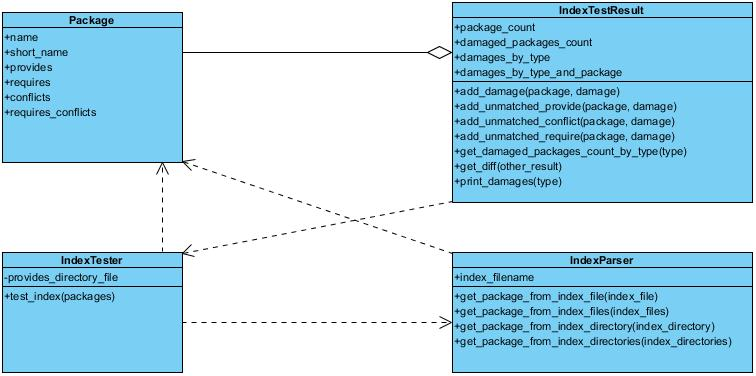
\includegraphics[scale=0.6, clip]{../resources/uml/ds_test_class_diagram.jpg}
\caption{Диаграмма классов модуля ds\_test.py}
\label{gr:dstestclassdiag}
\end{center}
\end{figure}

\textit{Package} - это класс, объекты которого представляют отдельные пакеты и, как видно из диаграммы,
содержат информацию а пакете, если сопоставлять: полю \textit{name} соответствует строка, заключенная
в квадратные скобки, полю \textit{short\_name} - строка, идущая ниже, а \textit{provides}, \textit{requires}
и \textit{conflicts} - это массивы строк, соответствующие одноименным множествам пакета. \\

Класс \textit{IndexParser} отвечает за разбор файлов индекса, в качестве параметра конструктора
ожидается файл, который необходимо обработать. Метод \textit{\_append\_index\_filename} получает на вход
имя директории с целевым файлом и образует из него и имени файла для парсинга
путь.\\
Основным методом класса \textit{IndexParser} является \textit{get\_packages\_from\_index\_file}.
В качестве входных данных используется сформированный ранее путь к файлу с данными
для парсинга. Этот метод возвращает генератор массива объектов класса \textit{Package.}\\

Тот факт, что метод \textit{get\_packages\_from\_index\_file} возвращает генератор позволяет
его использовать в том числе и для парсинга сразу нескольких файлов. Это происходит
в методе \textit{get\_packages\_from\_index\_files}, который на вход получает массивов файлов, 
затем для каждого файлы вызывает предыдущий метод. Этот метод так же возвращает
генератор массива объектов класса \textit{Package}.\\

Класс \textit{IndexTestResult} предназначен для удобной работы с результатами тестирования. 
У этого класса есть три метода отвечающие за накопление результатов тестирования:
\textit{add\_unmatched\_provide}, \textit{add\_unmatched\_require} и \textit{add\_unmatched\_conflict}, каждый из которых
в качестве первого аргумента получает объект класса \textit{Package} - текущий пакет, а в качестве второго
- строку, соответствующую повреждению(из множества \textit{provides}, \textit{requires} или \textit{conflicts}).
Для управления выводом переопределен метод \textit{\_\_str\_\_}. Так же у класса существует метод \textit{diff},
принимающий в качестве аргумента объект класса \textit{IndexTestResult}. Назначение метода 
заключается в том, чтобы при существовании двух результатов тестирования (объектов
класса \emph{IndexTestResult}) второй содержал только новые повреждения, то есть отсутствующие
в первом.\\

В классе \textit{IndexTester} определены методы, непосредственно отвечающие за тестирование
индекса. При создании объекта данного класса в конструкторе передается файл с директориями,
в которых может находится \textit{provide}, не считаясь избыточным. 
Алгоритм тестирования реализован в методе \textit{test\_index}. Этот метод на вход
получает массив объектов класса \textit{Package}. Алгоритм выглядит следующим образом:
\begin{enumerate}
\item{Инициализация списка имен пакетов - \textit{names\_set}, списка \textit{provides} и 
списка \textit{requires\_conflicts}}
\item{Совершается проход в цикле по всем пакетам. На каждом шаге 
к уже сформированным спискам \textit{provides}, \textit{requires\_conflicts} и \textit{names\_set} 
добавляются данные пакета. В результате получаем набор списков всех \textit{provides}, 
\textit{requires\_conflict} и имен для набора пакетов}
\item{Создается объект класса \textit{IndexTestResult}}
\item{Совершается проход в цикле по всем пакетам. На каждом шаге цикла проверяется}
\end{enumerate}
\begin{itemize}
\item{Для каждого \textit{provide} пакета проверяется является ли он избыточным: существует ли
строка из списка \textit{requires\_conflicts} или находится ли он в одной из заданных директорий.
Если не является, то данный пакет помечается, как поврежденный, а данный provide помечается,
как избыточный, то есть вызывается метод \emph{add\_unmatched\_provide} у объекта класса \textit{IndexTestResult}}
\item{Для каждого \textit{require} пакета проверяется не является ли он анметом: существует ли
соответствующая строка из списка \textit{provides}. Если не существует, то пакет помечается, как 
поврежденный, а \textit{require}, как \textit{анмет}, то есть вызывается метод \textit{add\_unmatched\_require}
у объекта класса \textit{IndexTestResult}}
\item{Для каждого \textit{conflict} пакета проверяется не является ли он избыточным: существует ли
соответствующая строка из списка \textit{provides}. Если не существует, то пакет помечается, как 
поврежденный, а \textit{conflict}, как поврежденный, то есть вызывается метод \textit{add\_unmatched\_conflict}
у объекта класса \textit{IndexTestResult}}

\item{Возвращается объект класса \textit{IndexTestResult}}
\end{itemize}

\subsection{Утилита для проверки готового индекса}
Для тестирования целостности репозитория используются данные из файла \textit{rpms.data},
в котором описание каждого пакета соответствует следующему формату:
\begin{itemize}
\item{[name-version-release.architecture.rpm] }
\item{n=name} 
\item{e=epoch}
\item{v=version}
\item{r=release}
\item{arch=architecture}
\item{btime=build time}
\item{p:provide}
\item{r:require}
\item{c:conflict}
\item{o:obsolete}
\end{itemize}
Очевидно, что каждому пакету соответствует набор множеств \textit{provides},
\textit{requires}, \textit{conflicts}, \textit{obsoletes}, которые могут быть и пустыми.\\

Под целостностью репозитория понимается состояние, которое удовлетворяет следующим
условиям:
\begin{itemize}
\item{Для каждого \textit{require} пакета существует одноименный \textit{provide} 
другого пакета. Require, для которого это условие не выполняется
называется \textit{анметом (unmet)}. }
\item{Для каждого \textit{provide} существует одноименный \textit{require/conflict} или
он находится в директории из заранее заданного списка.Это условие 
контролирует появление избыточных \textit{provide}, засчет которых %%FIXME:сделать ссылку на место, где про это говорилось
может существенно расти размер индекса.}
\item{Для каждого \textit{conflict} пакета существует одноименный \textit{provide} 
другого пакета. Это условие не является таким строгим, как два предыдущих,
но желательно, чтобы оно выполнялось. }
\end{itemize}

В качестве входных данных используется файл с содержимым формата, описанного выше,
и расширением \textit{*.data.gz}.

Таким образом, первый этап проверки сводится к выполнению следующих действий:
\begin{itemize}
\item{Создание объектов класса \textit{IndexParser} и \textit{IndexTester}.}
\item{Создание и заполнение массива объектов класса \textit{Package} при помощи
вызова метода \textit{get\_packages\_from\_index\_files} у объекта класса \textit{IndexParser}.}
\item{Получение результатов тестирования посредством вызова метода \textit{test\_index}
у объекта класса \textit{IndexTester}}
\end{itemize}

На выходе получается статистика вида:\\
\\
Found [количество найденных пакетов] packages\\
.[количество поврежденных пакетов] packages are damaged\\
.[количество пакетов с избыточными provide] packages have unmatched provides\\
.[количество пакетов с анметами] packages have unmets\\
.[количество пакетов с избыточными conflict] packages have unmatched conflicts\\

Подробная информация о повреждениях регулируется с помощью ключей и имеет следующий формат:\\
package [имя пакета] has unmatched [тип: provide или conflict] [строка соответствующая повреждению]\\
package [имя пакета] has [тип: unmet] [строка соответствующая повреждению]\\

\subsection{Проверка утилит для обновления индекса}
Для данной проверки в качестве входных данных необходимо предоставить
путь до каталога \textit{base.*}, так как утилиты \textit{ds-patch} и 
\textit{ds-provides} используют данные всех файлов из директории.\\
Под утилитами для обновления индекса подразумеваются описанные
выше \textit{ds-patch} и \textit{ds-provides}.

Проверка представляет собой последовательность действий:\\
\begin{itemize}
\item{Проведение начального тестирования на неизменном индексе. Сохранение
и вывод результатов.}
\item{Совершаем проход в цикле по каждой директории из \emph{INDEX\_FILES\_PATH}. На
каждом шаге:
	\begin{itemize}
	\item{Формируем список пакетов для текущей директории.}
	\item{Для каждого пакета из списка вызывается утилита \textit{ds-patch }
	для текущего пакета, затем \textit{ds-provides} для директории файла, а 
	так же связанных с ней. После этого проводится тестирование
	измененного индекса и вывод результатов отличных от начальных
	с использование метода \textit{diff} объекта класса \textit{IndexTestResult}.}
	\end{itemize}
}
\end{itemize}

В качестве результата данная утилита предоставляет статистику выше описанного формата,
полученную сначала на готовом индексе, а затем после каждого запуска утилит для обновления
индекса. Отображение выходных данных этой утилиты так же регулируется ключами.









\newpage


\newpage
\section*{Заключение}
\addcontentsline{toc}{section}{\hspace{7mm}Заключение}
В результате настоящей работы были достигнуты поставленные цели:
\begin{itemize}
\item{Изучен механизм дистрибуции программного обеспечения в операционных системах Linux.}
\item{Произведено знакомсто с основными проблемами в этой сфере и способами их решения.}
\item{Создан программные продукт для тестирования целостности репозитория Deepsolver.}
\end{itemize}
Тестирование проводилось для проверки индексов репозитория пакетного менеджера \textit{Deepsolver}.
В течение года производились многократные отладки процедуры обновления индекса, контроль
за влиянием изменений проводился с помощью данных утилит.
На данный момент индексы \textit{Deepsolver} интегрированы в официальный репозиторий
компании \textit{ALT Linux}. Описанные в настоящей работе утилиты были применены для 
проверки целостности индекса, на настоящий момент находящегося в промышленном применении.


\newpage

\addcontentsline{toc}{section}{\hspace{7mm}Список использованных источников и литературы}
\begin{thebibliography}{0}
\bibitem{dependencies_model}
Burrows,~D.~,
Modelling and Resolving Software Dependencies /
Daniel Burrows //
Conferenza Italiana sul Software Libero (CONFSL, 2005)

\bibitem{deepsolver_ta}
Приложение для управления rpm-пакетами и контроля целостности операционной системы. Техническое задание 
--- \url{http://deepsolver.altlinux.org/tech-assignment.pdf} // Альт Линукс --- 2012

\bibitem{deepsolver_um}
Deepsolver --- менеджер пакетов. Руководство пользователя
--- \url{http://deepsolver.altlinux.org/user-manual.pdf}. // Альт Линукс --- 2013

\bibitem{apt_pbo}
Trezentos~P.~
Apt-pbo: solving the software dependency problem using pseudo-boolean optimization /
Paulo Trezentos, Ines Lynce, and Arlindo L. Oliveira //
ASE 2010, September 20-24, 2010, Antwerp, Belgium.

\end{thebibliography}
\newpage

\end{document}
